
%%%%%%%%%%%%%%%%%%%%%%%%%%%%%%%%%%%%%%%%%%%%%%%%%%%%%%%
%Figure
%%%%%%%%%%%%%%%%%%%%%%%%%%%%%%%%%%%%%%%%%%%%%%%%%%%%%%%
%\begin{landscape}

\begin{figure}[H]
	\caption{Treatment dynamics (all deals) \newline
		The figure presents the dynamics of treatment over time. Outcome variable is the log of dealsize across all three categories (loans, bonds, SEOs). Vertical bars represent 90\% confidence intervals for standard errors clustered at firm and lender. The year of treatment is the first year in which a banker appears on a loan for a new bank.} 
	\label{fig:dynamics_full}
	\centering
	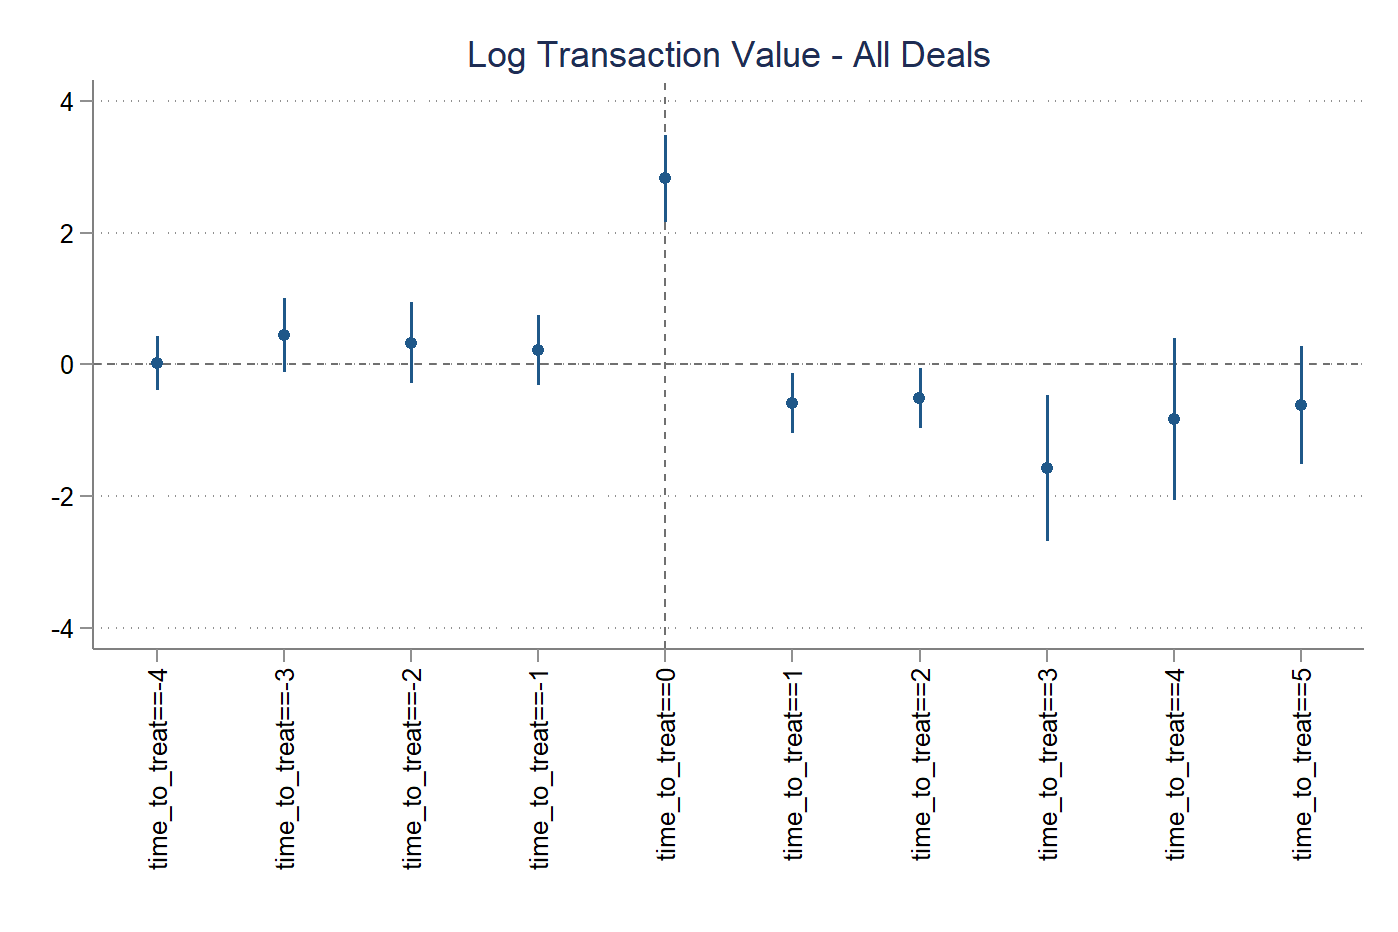
\includegraphics[angle=0,  scale=0.35]{figures/dynamics_logdealsize.png}
\end{figure}
%\end{landscape}

\clearpage \newpage

%%%%%%%%%%%%%%%%%%%%%%%%%%%%%%%%%%%%%%%%%%%%%%%%%%%%%%%
%Figure
%%%%%%%%%%%%%%%%%%%%%%%%%%%%%%%%%%%%%%%%%%%%%%%%%%%%%%%

\begin{figure}[H]
	\caption{Treatment dynamics  (bonds only) \newline
		The figure presents the dynamics of treatment over time. Outcome variable is the log of dealsize of new bonds issued. Vertical bars represent 90\% confidence intervals for standard errors clustered at firm and lender. The year of treatment is the first year in which a banker appears on a loan for a new bank.} 
	\label{fig:dynamics_bonds}
	\centering
	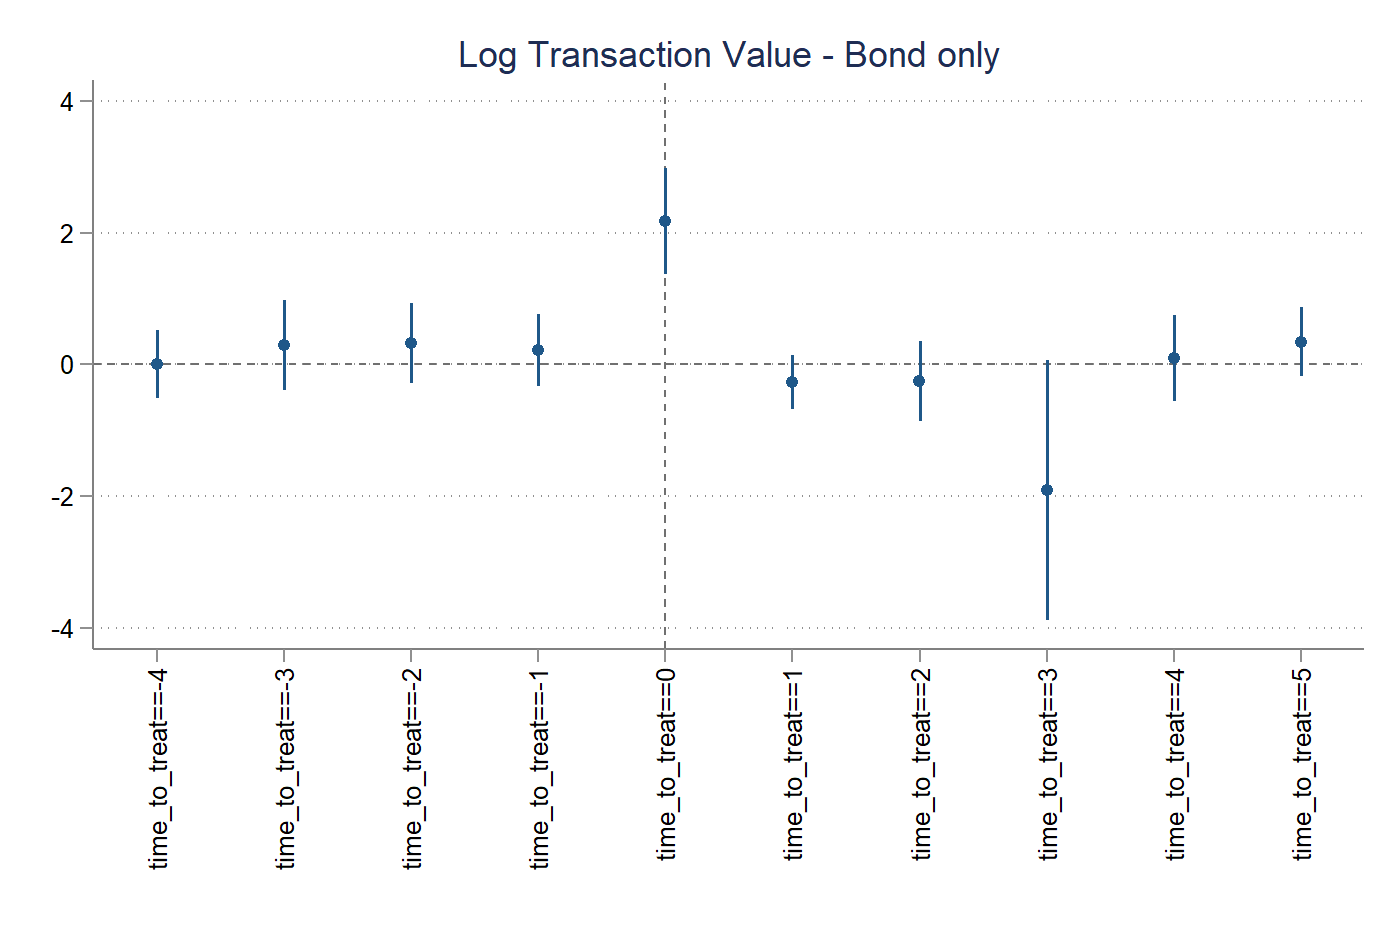
\includegraphics[angle=0,  scale=0.35]{figures/dynamics_logdealsize_bondonly.png}
\end{figure}
%\end{landscape}

\clearpage \newpage

%%%%%%%%%%%%%%%%%%%%%%%%%%%%%%%%%%%%%%%%%%%%%%%%%%%%%%%
%Figure
%%%%%%%%%%%%%%%%%%%%%%%%%%%%%%%%%%%%%%%%%%%%%%%%%%%%%%%


\begin{figure}[H]
	\caption{Treatment dynamics (SEO only) \newline
		The figure presents the dynamics of treatment over time. Outcome variable is the log of dealsize of seasoned equity offerings. Vertical bars represent 90\% confidence intervals for standard errors clustered at firm and lender. The year of treatment is the first year in which a banker appears on a loan for a new bank.} 
	\label{fig:dynamics_seo}
	\centering
	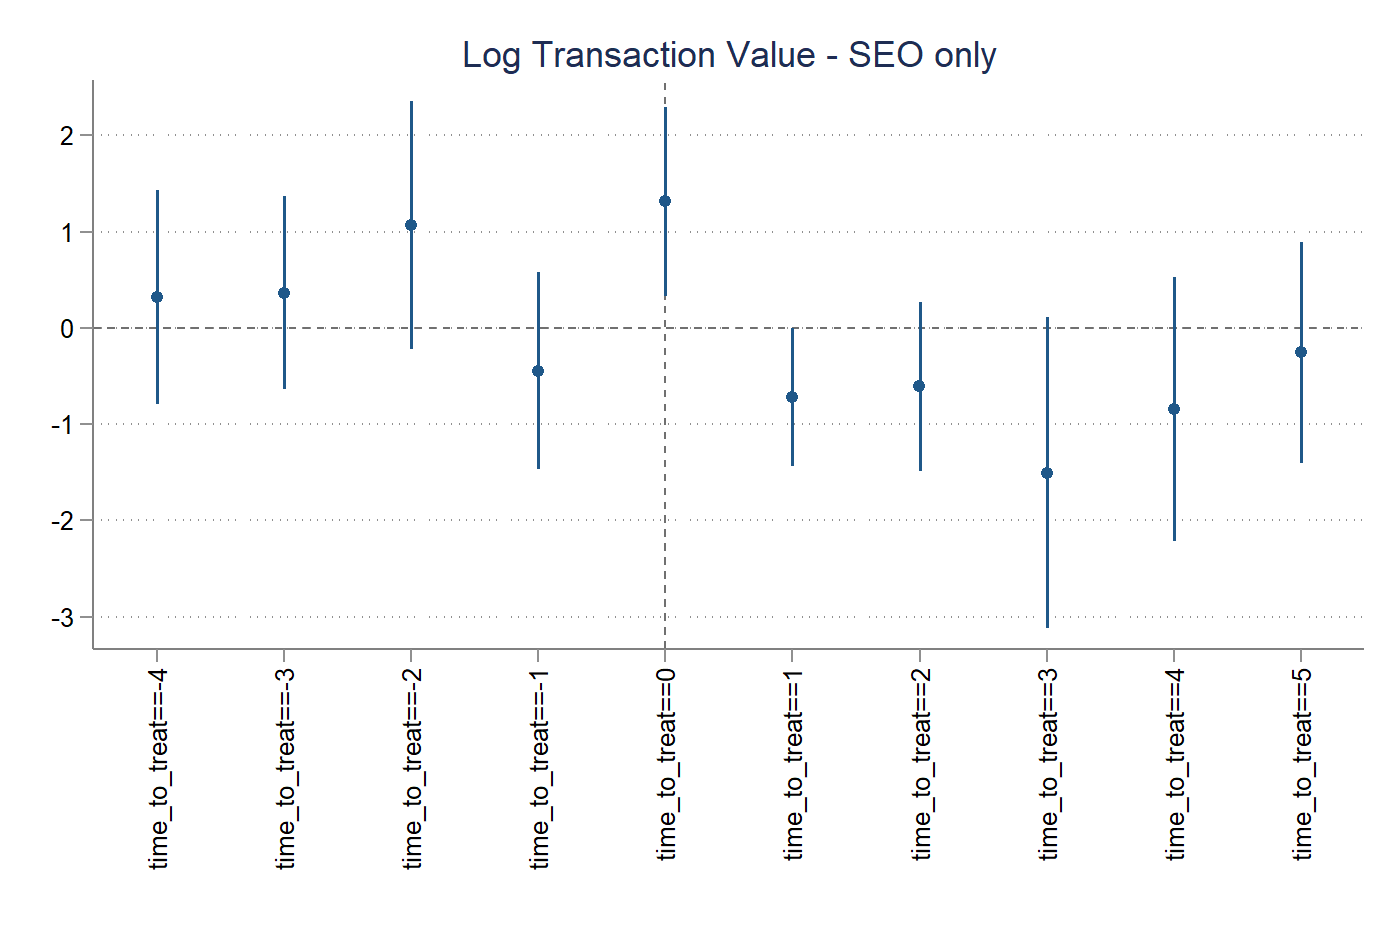
\includegraphics[angle=0,  scale=0.35]{figures/dynamics_logdealsize_seoonly.png}
\end{figure}
%\end{landscape}

\clearpage \newpage

\begin{figure}[H]
\captionsetup[subfigure]{justification=centering}
	\centering
	\caption{\textbf{Treatment dynamics - First deal and repeat business} \newline The figure presents the dynamics of treatment over time. Outcome variable in Panel A is the log of dealsize of the first deal (either syndicated loan, bond underwriting, or seasoned equity offering) in which a banker appears on a loan for a new bank. Panel B shows the total transaction value of repeated business done with a client (except for the first deal). Vertical bars represent 90\% confidence intervals for standard errors clustered at firm and lender. The year of treatment is the first year in which a banker appears on a loan for a new bank.} 
	\label{fig:dynamics_first_repeated}
	\begin{subfigure}[H]{\textwidth}
		\centering
		\caption*{\textbf{Panel A:} Log Transaction Value - First deal of old clients at new bank}
		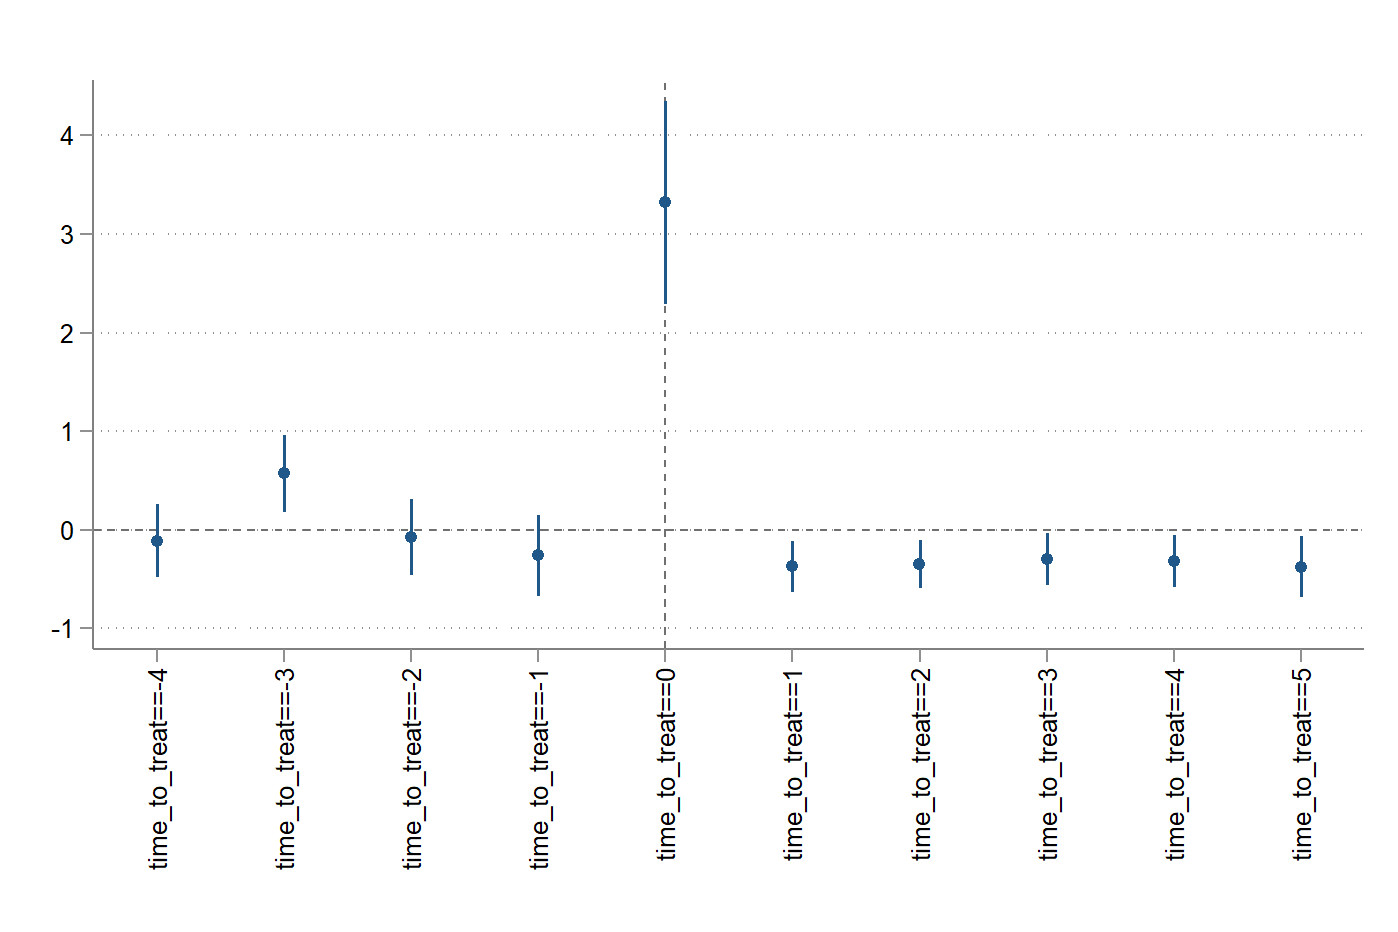
\includegraphics[angle=0,  scale=0.3]{figures/dynamics_logdealsize_firsttime.png}
		\caption*{[Continued on the next page]}
	\end{subfigure} \end{figure}

\begin{figure}[H]
\captionsetup[subfigure]{justification=centering}
	{\small \centering [Continued from previous page] \\ ~ \newline}
	\begin{subfigure}[H]{\textwidth}
		\centering
		\caption*{\textbf{Panel B:} Log Transaction Value - Repeat business with old clients at new bank}
		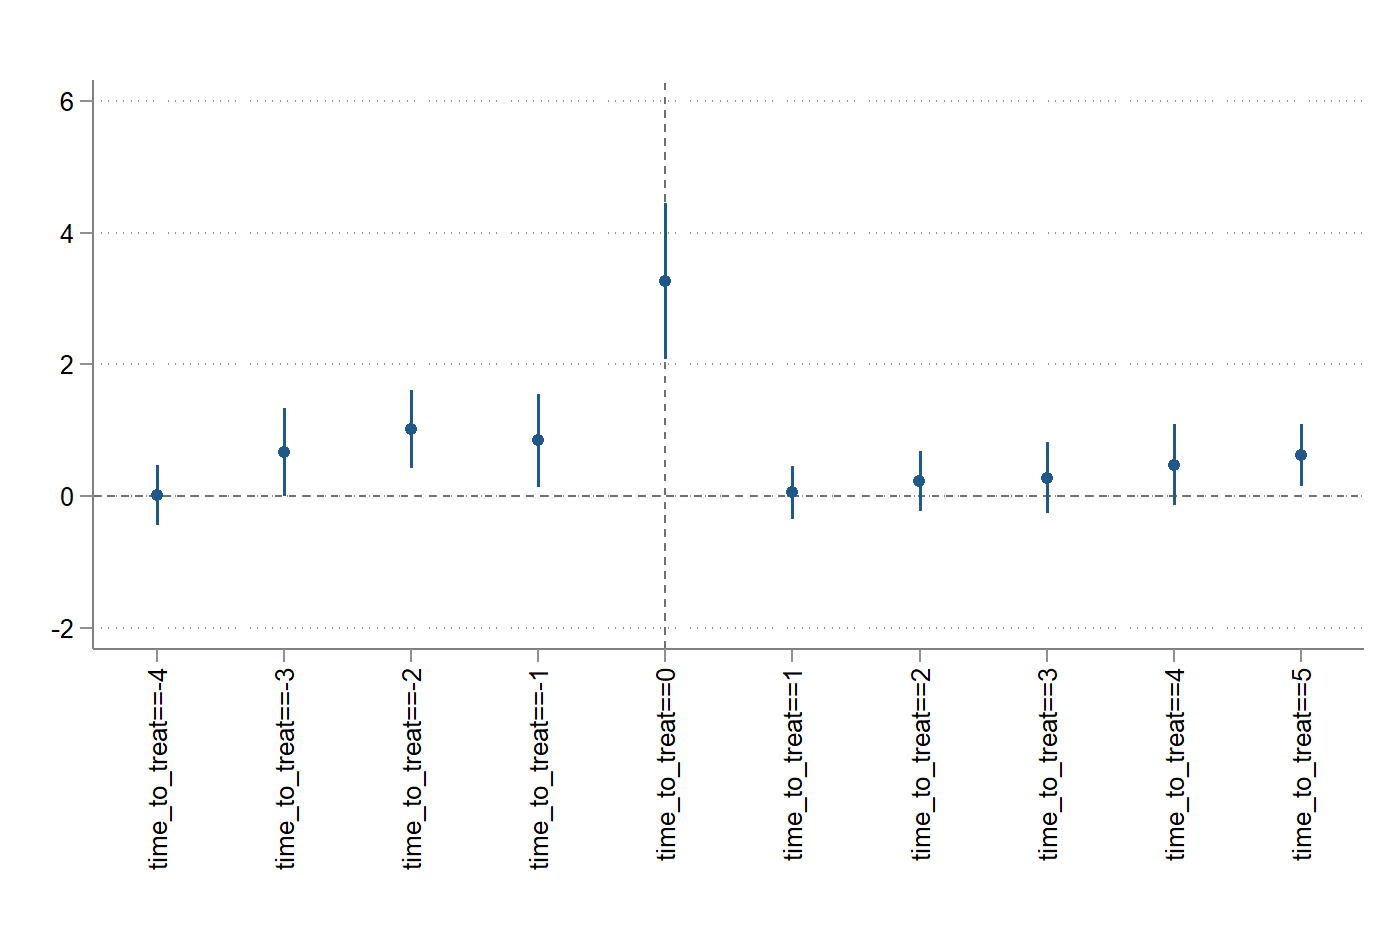
\includegraphics[angle=0,  scale=0.3]{figures/dynamics_logdealsize_repeat.png}
	\end{subfigure}
\end{figure}

%%%%%%%%%%%%%%%%%%%%%%%%%%%%%%%%%%%%%%%%%%%%%%%%%%%%%%%
%Figure
%%%%%%%%%%%%%%%%%%%%%%%%%%%%%%%%%%%%%%%%%%%%%%%%%%%%%%%